\documentclass{beamer}
\usepackage[utf8]{inputenc}
\usepackage{color}
\usepackage{geometry}
\usepackage{tikz}
\usetheme{Madrid}
\title{Sorting}
\subtitle{An Introduction}
\author[Ayesha] {Ayesha Binte Mostofa}
\institute[BUET]{
Department of Computer Science and Engineering\\
Bangladesh University of Engineering and Technology}
\date{\today}

\begin{document}

\frame{\titlepage}

\begin{frame}{Table of Contents}
    \tableofcontents
\end{frame}

\section{Introduction}
\begin{frame}{Sorting}
\begin{itemize}
    \item[] {\color{blue}Insertion sort }a sorting algorithm that places an unsorted element at its suitable place in each iteration\pause
    \item[] {\color{blue}Bubble sort} a sorting algorithm that compares two adjacent elements and swaps them until they are in the intended order
\end{itemize}
\end{frame}

\begin{frame}{Features}
    \begin{alertblock}{Time Complexity}
    O($n^2$)
    \end{alertblock}
\end{frame}


\tikzstyle{greyt}=[rectangle,draw=blue!50,fill=black!20,thick]
\tikzstyle{bluet}=[rectangle,draw=blue!50,fill=blue!20,thick]
\tikzstyle{whitet}=[rectangle,draw=blue!50,fill=white!20,thick]

\section{Insertion Sort}
\begin{center}
\begin{frame}{Insertion Sort}
\begin{tikzpicture}
\node at (4,5) [greyt] {1};
\node at (5,5) [bluet] {10};  
\node at (6,5) [whitet] {7};
\node at (7,5) [whitet] {-100};  
\node at (8,5) [whitet] {3};
\end{tikzpicture}
\end{frame}

\begin{frame}{Insertion Sort}
\begin{tikzpicture}
\node at (4,5) [greyt] {1};
\node at (5,5) [greyt] (r) {10};  
\node at (6,5) [bluet] (b) {7};
\draw [->] (b) to [out=90,in=90] (r);
\node at (7,5) [whitet] {-100};  
\node at (8,5) [whitet] {3};
\end{tikzpicture}
\end{frame}

\begin{frame}{Insertion Sort}
\begin{tikzpicture}
\node at (4,5) [greyt] {1};
\node at (5,5) [greyt] {7};  
\node at (6,5) [bluet] {10};
\node at (7,5) [whitet] {-100};  
\node at (8,5) [whitet] {3};
\end{tikzpicture}
\end{frame}

\begin{frame}{Insertion Sort}
\begin{tikzpicture}
\node at (4,5) [greyt] (r) {1};
\node at (5,5) [greyt]  {7};  
\node at (6,5) [greyt]  {10};
\node at (7,5) [bluet] (b) {-100};  
\node at (8,5) [whitet] {3};
\draw [->] (b) to [out=90,in=90] (r);
\end{tikzpicture}
\end{frame}

\begin{frame}{Insertion Sort}
\begin{tikzpicture}
\node at (4,5) [greyt] {-100};
\node at (5,5) [greyt]  {1};  
\node at (6,5) [greyt]  {7};
\node at (7,5) [bluet] {10};  
\node at (8,5) [whitet] {3};
\end{tikzpicture}
\end{frame}

\begin{frame}{Insertion Sort}
\begin{tikzpicture}
\node at (4,5) [greyt] {-100};
\node at (5,5) [greyt]  {1};  
\node at (6,5) [greyt]  (b) {7};
\node at (7,5) [greyt] {10};  
\node at (8,5) [bluet] (r) {3};
\draw [->] (r) to [out=90,in=90] (b);
\end{tikzpicture}
\end{frame}

\begin{frame}{Insertion Sort}
\begin{tikzpicture}
\node at (4,5) [greyt] {-100};
\node at (5,5) [greyt]  {1};  
\node at (6,5) [greyt]  {3};
\node at (7,5) [greyt] {7};  
\node at (8,5) [bluet] {10};
\end{tikzpicture}
\end{frame}

\begin{frame}{Insertion Sort}
\begin{tikzpicture}
\node at (4,5) [greyt] {-100};
\node at (5,5) [greyt]  {1};  
\node at (6,5) [greyt]  {3};
\node at (7,5) [greyt] {7};  
\node at (8,5) [greyt] {10};
\end{tikzpicture}
\end{frame}

\section{GRID}
\begin{frame}{GRID}
    \begin{tikzpicture}
    \draw[help lines] (0,0) grid (5,5);\pause
    \draw[->](0,0)--(0,6);\pause
    \draw[thick][->](0,0)--(6,0);\pause
    \node [above left] at (0,6) {Y};\pause
    \node [below right] at (6,0) {X};\pause
    \foreach \x in {0,...,5}
        \node at (\x+0.5, -0.25) {\x};\pause
    \foreach \y in {0,...,5}
        \node at (-.5, \y+0.25) {\y};
    \end{tikzpicture}
\end{frame}

\begin{frame}{Figure}
\begin{figure}
    \centering
    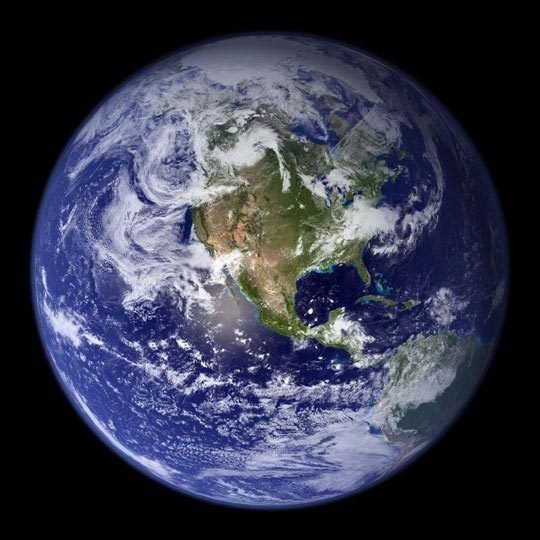
\includegraphics[height = 5cm]{e.jpg}
    \caption{Caption}
    \label{fig:my_label}
\end{figure}
\end{frame}
    
\end{center}
\end{document}
